\section{Il web in numeri: statistiche}
Se si da uno sguardo alle statistiche ci si può accorgere che la maggior parte dei siti non dedica le giuste attenzioni all'ottimizzazione del proprio servizio, in particolare secondo uno studio effettuato da tooltester.com:
\begin{itemize}
    \item Il tempo di caricamento medio delle pagine è di 2.5 secondi per i device desktop e 8 per i device mobile.
    \item Il delay del primo contatto con l'utente è di 12.73 millisecondi per i device desktop e di 59.73 per i device mobile
    \item Le pagine  impiegano un tempo medio di caricamento superiore del 70.9\% su device mobile rispetto che su device desktop
    \item Gli utenti di device mobile sono al primo posto nella classifica di abbandono delle pagine con una percentuale di 56.8\% 
    \item il settore delle scienze possiede il rateo di abbandono più alto con una percentuale di 66.37\%
    \item Di tutte le tipologie di device (desktop/tablet/mobile) il tablet è quello con il minor numero di sessioni all'anno con una percentuale di 2.3%
\end{itemize}
\begin{figure}[H]
   \centering
   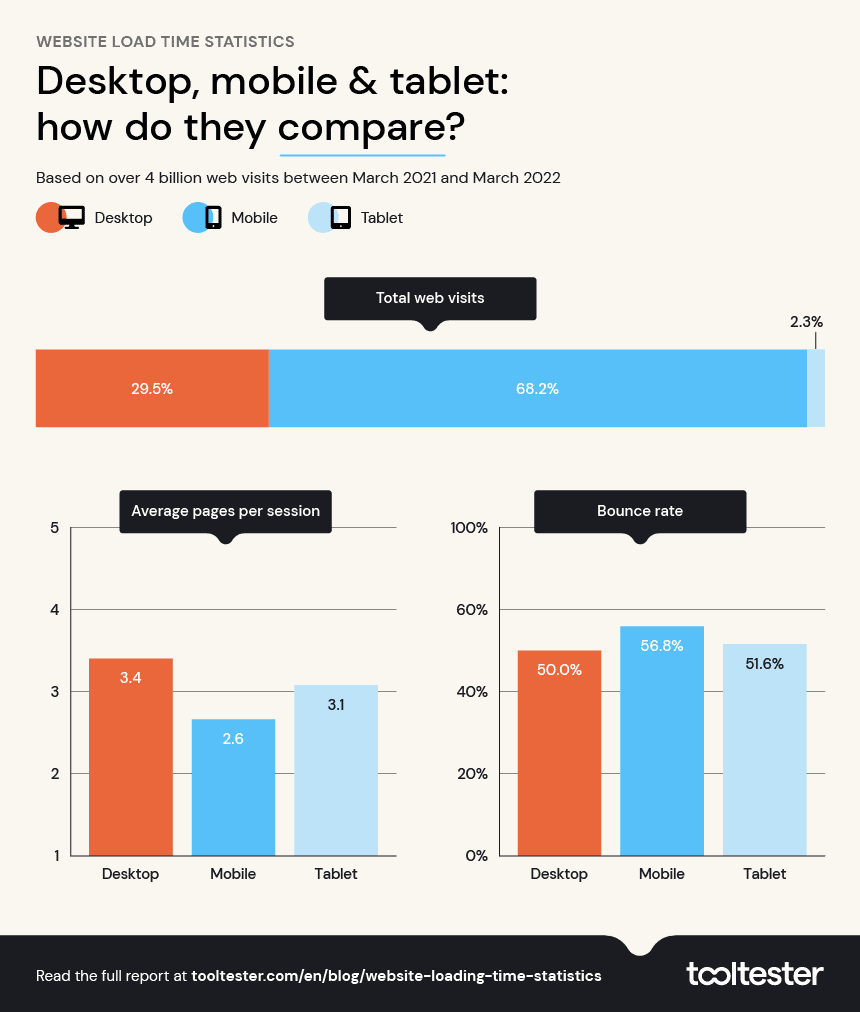
\includegraphics[scale=0.25]{resources/website-load-time-statistics-desktop-mobile-tablet.png}
\cite{website-loading-time-statistics}
\caption{Statistiche di visualizzazione pagine web}
\end{figure}


   